\documentclass{article}

\usepackage{inputenc}[utf8]
\usepackage[T1]{fontenc}
\usepackage{url}
\usepackage{hyperref}
\usepackage[ngerman]{babel}
\usepackage{graphicx}

\usepackage{amsmath}

\title{{\Huge Aufgabenblatt 02}\\Einführung in die Kryptographie PS}
\author{Andreas Schlager}

\begin{document}
    \maketitle
    \tableofcontents
    \section{Aufgabe 6}
    \textit{Erklären Sie, warum bei Hamming ECC (Error Correction Code) die Parity Bits zwischen den Datenbits
    eingefügt werden und nicht einfach alle geschlossen den Datenbits vorangestellt oder
    angehängt werden. Illustrieren Sie das anhand eines Beispiels unter Verwendung
    eines (15,11)-Hamming Codes.}\vspace*{1em}\newline
    In einer Hamming-codierten Nachricht befinden sich die Paritätsbits nicht am Anfang oder Ende der Nachricht, 
    sondern an speziellen Positionen, die Zweierpotenzen entsprechen (z.B. $1, 2, 4, 8, \dots$).
    Sie zeichnen sich dadurch aus, dass ihre Binärdarstellung genau eine gesetzte 1 hat.
    \begin{center}
        \begin{tabular}{c|c} 
            \textbf{Position} & \textbf{Binärdarstellung}\\\hline
            1 & 000001\\
            2 & 000010\\
            4 & 000100\\
            8 & 001000\\
            16 & 010000\\
            32 & 100000
        \end{tabular}
    \end{center}
    Diese Eigenschaft ermöglicht eine effiziente Fehlererkennung und -korrektur durch eine XOR-Verknüpfung.
    Da die Einsen an unterschiedlichen Positionen sind, beeinflussen sie sich später in der Berechnung nicht gegenseitig.
    Wird eine entsprechende Wahl der Paritätsbits getroffen (odd oder even), dann ergibt die XOR-Verknüpfung 
    aller Positionen, an denen eine Eins steht, stets null wenn kein Fehler aufgetreten ist. Ansonsten ist das 
    Ergebnis die Position des Bits, welches fehlerhaft übertragen wurde. Falls mehrere Bits gekippt sind, 
    entsteht zumindest ein unerwartetes Ergebnis. Dadurch ist zwar erkennbar, dass ein Fehler vorliegt, 
    er kann jedoch nicht behoben werden.
    \subsection{Beispiel Hamming(15,11)}
    Angenommen man möchte das Datenwort $10110111011_2$ übertragen und durch einen Hamming ECC absichern,
    dann würde die ganze Nachricht mit den Paritätsbits wie folgt aussehen:
    \begin{center}
        \begin{tabular}{l|ccccccccccccccc}
            \textbf{Position} & 1 & 2 & 3 & 4 &5&6&7&8&9&10&11&12&13&14&15\\\hline
            \textbf{Nachricht} & $P_1$ & $P_2$ & 1 & $P_3$ &0&1&1&$P_4$& 0 & 1 & 1& 1 &0 & 1 & 1
        \end{tabular}
    \end{center}
    Das Ziel ist eine Auswahl der Paritätsbits in Abhängigkeit der Position mit Einsen, sodass eine XOR-Verknüpfung
    der Positionen Null ergibt. Die Paritätsbits beeinflussen sich in der Berechnung nicht gegenseitig, da eben alle
    eine Zweierpotenz als Stelle haben. Für das Beispiel versucht man nun spaltenweise eine geeignete Auswahl der Bits
    zu treffen. Dafür schreibt man alle Positionen an denen Einsen 
    auftreten in Binärdarstellung untereinander auf.
    \[
    \begin{array}{c c c}
        \begin{tabular}{c|cccc}
            Position & $b_4$ & $b_3$ & $b_2$ & $b_1$\\\hline
            3 & 0 & 0 & 1 & 1\\
            6 & 0 & 1 & 1 & 0\\
            7 & 0 & 1 & 1 & 1\\
            10 & 1 & 0 & 1 & 0\\
            11 & 1 & 0 & 1 & 1\\
            12 & 1 & 1 & 0 & 0\\
            14 & 1 & 1 & 1 & 0\\
            15 & 1 & 1 & 1 & 1\\\hline
            Parity & $P_4$ & $P_3$ & $P_2$ & $P_1$\\\hline
            XOR & 0 & 0 & 0 & 0
        \end{tabular} &\Longrightarrow&
        \begin{tabular}{c|cccc}
            Position & $b_4$ & $b_3$ & $b_2$ & $b_1$\\\hline
            3 & 0 & 0 & 1 & 1\\
            6 & 0 & 1 & 1 & 0\\
            7 & 0 & 1 & 1 & 1\\
            10 & 1 & 0 & 1 & 0\\
            11 & 1 & 0 & 1 & 1\\
            12 & 1 & 1 & 0 & 0\\
            14 & 1 & 1 & 1 & 0\\
            15 & 1 & 1 & 1 & 1\\\hline
            Parity & 1 & 1 & 1 & 0\\\hline
            XOR & 0 & 0 & 0 & 0
        \end{tabular}
    \end{array}
    \]
    Die vollständige Nachricht lautet somit:
    \begin{center}
        \begin{tabular}{l|ccccccccccccccc}
            \textbf{Position} & 1 & 2 & 3 & 4 &5&6&7&8&9&10&11&12&13&14&15\\\hline
            \textbf{Nachricht} & $0$ & $1$ & 1 & $1$ &0&1&1&$1$& 0 & 1 & 1& 1 &0 & 1 & 1
        \end{tabular}
    \end{center}
    Die Wahl der Paritätsbits führt zu einer Gleichung der folgenden Form, wobei $B(n)$ die Binärdarstellung
    von $n$, $\oplus$ die XOR-Verknüpfung ist.
    \[
        B(3) \oplus \cdots\oplus B(15) \oplus B(8) \oplus B(4) \oplus B(2) = 0_2
    \]
    Die Position $8, 4, 2$ sind vorhanden, weil die Paritätsbits $P_4, P_3, P_2$ laut Tabelle Eins sein müssen.
    Würde nun ein Bit $x$ bei der Übertragung kippen, gäbe es zwei Fälle. Einerseits könnte eine Null zu einer Eins geworden
    sein, wodurch in der Berechnung eine zusätzliche Stelle $B(x)$ hinzu kommt. Dadurch würde der Empfänger folgendes
    Ergebnis erhalten:
    \begin{align*}
        B(3) \oplus \cdots\oplus B(15) \oplus B(8) \oplus B(4) \oplus B(2)\oplus B(x) &=\\
        0_2 \oplus B(x) &= B(x)
    \end{align*}
    Also genau die Stelle an der ein Fehler passiert ist. Andererseits könnte auch eine Eins zu einer Null geworden
    sein. Dadurch fehlt genau ein Term auf der linken Seite, um das Ergebnis Null zu erhalten. Angenommen $B(x) = B(3)$. 
    \begin{align*}
        B(6) \oplus \cdots\oplus B(15) \oplus B(8) \oplus B(4) \oplus B(2) = 0_2 \oplus B(3) = B(3)
    \end{align*}
    Dadurch könnte der Empfänger den Fehler an der Stelle $3$ beheben.
    \section{Aufgabe 7}
    \textit{Erklären Sie, warum es allgemein schwierig ist, aus biometrischen Messungen kryptographisches 
    Schlüsselmaterial zu gewinnen. Illustrieren Sie das ganz konkret anhand der Features/Merkmale
    einer bestimmten biometrischen Modalität (also wie würde man konkret einen Schlüssel
    generieren und was ist das Problem).}\vspace*{1em}\newline
    Ein wichtiges Merkmal eines guten kryptographischen Systems ist, dass eine kleine Änderung des Schlüssels
    zu einem komplett anderem Ciphertext führt. Registriert man nun ein biometrisches Merkmal durch eine Messung, 
    um daraus einen  Schlüssel zu erzeugen, ist es daher wichtig bei jeder weiteren Messung des gleichen Merkmals 
    auch wieder den gleichen Schlüssel zu generieren. Andernfalls wird die Authentifizierung scheitern. Wie man
    aus der Messlehre allerdings weiß, sind kleine Messungenauigkeiten unumgänglich.
    \subsection{Fingerabdruck-Schlüssel}
    Fingerabdrücke sind bei jedem Menschen einzigartig und bieten sich daher zur biometrischen Authentifizierung an.
    Um von einem Fingerabdruck einen kryptographischen Schlüssel zu generieren, gibt es mehrere Schritte:
    \begin{enumerate}
        \item Über einen optischen Fingerabdruck-Scanner wird ein Bild des Fingers erfasst. Dafür wird
        die Fingerfläche beleuchtet, um Hebungen und Vertiefungen sichtbar zu machen.
        \item Aus dem Bild werden Merkmale wie die Positionen, die Winkel und die Verzweigungen der Fingerlinien extrahiert.
        Diese Merkmale werden auch \textbf{Minutien} genannt.
        \item Die Minutien-Werte werden in eine strukturierte Form gebracht und in binärer Darstellung als Schlüssel interpretiert.
    \end{enumerate}
    Das Problem entsteht dann, wenn der Scanner zwangsläufig leicht unterschiedliche Merkmale wahrnimmt. Je nach 
    Druck oder Position des Fingers werden die Messungen beeinflusst und unterscheiden sich dementsprechend voneinander.
    In weitere Folge würde sich der Schlüssel ebenfalls leicht unterscheiden, wodurch der/die Nutzer:in nicht
    authentifiziert werden würde. Um eine größere Zuverlässigkeit zu erzielen, können bei der Registrierung 
    zusätzlich Fehlerkorrekturdaten gespeichert.
    \section{Aufgabe 8}
    \textit{Erklären Sie das Fuzzy Commitment Scheme zur Erzeugung von kryptographischen Schlüsseln aus 
    biometrischen Messungen. Welche Rolle spielen dabei fehlerkorrigierende Codes? (siehe S.67f des 
    \href{https://www.cosy.sbg.ac.at/~uhl/biometrics_slides.pdf}{Biometrie Skriptums} \cite{Uhl2016})}\vspace*{1em}\newline
    Bei biometrischen Kryptosystemen spielt die Verwaltung der Schlüssel eine wichtige Rolle. Dafür gibt zwei
    Haupansätze: \textbf{Key-Generation Schemes} und \textbf{Key-Binding Schemes}.
    \subsection{Key-Generation Schemes}
    Bei Key-Generation Schemes werden die Ergebnisse der biometrischen Messung als Schlüssel interpretiert. Das bedeutet
    die biometrischen Merkmale dienen als Zufallsquelle für den \textbf{gesamten} Schlüssel. Dadurch müssen auch keine
    Schlüssel gespeichert werden, wodurch das System vereinfacht wird und kein sicheres Speicherkonzept notwendig ist.
    Allerdings muss bei jedem Authentifizierungsversuch der Schlüssel zu 100\% korrekt erzeugt werden, da sonst die 
    Authentifizierung fehlschlägt. Deshalb benötigt man zusätzliche Fehlerkorrekturdaten, um eine Toleranz bei der Messung
    zu erlauben. Außerdem gibt es ein Sicherheitsrisiko, da der gesamte Schlüssel aus den biometrischen Daten erzeugt werden
    kann. Sobald ein Angreifer eine verwertbare biometrische Probe hat, ist der Schlüssel dauerhaft komprimiert.
    \subsection{Key-Binding Schemes}
    Key-Binding Schemes verwenden einen, von den biometrischen Daten \textbf{unabhängigen}, Schlüssel. Der Schlüssel
    wird bei der Registrierung zufällig erzeugt, über eine Funktion an eine biometrische Probe gebunden und anschließend
    gespeichert. Über einen erneute Messung des Merkmals, den gespeicherten Daten und einem entsprechenden 
    Wiederherstellungsverfahren kann der Schlüssel zur Authentifizierung wieder erzeugt werden. Auch in diesem Fall
    wird in den gespeicherten Daten eine Form von fehlerkorrigierendem Code eingebettet um die Variationen 
    der Messung auszugleichen. Da in diesem Fall der Schlüssel unabhängigen ist, kann im Fall einer Komprimierung
    einfach ein neuer erzeugt werden.
    \subsubsection{Fuzzy Commitment Scheme}
    Das Fuzzy Commitment Scheme beinhaltet zwei Phasen: die Registrierung neuer Schlüsseldaten und die Verifikation über
    die Wiederherstellung des Schlüssel, durch eine biometrische Probe.
    \begin{figure}[h]
        \caption{Fuzzy Commitment Scheme Diagram (siehe \cite{Uhl2016}, S67)}
        \centering
        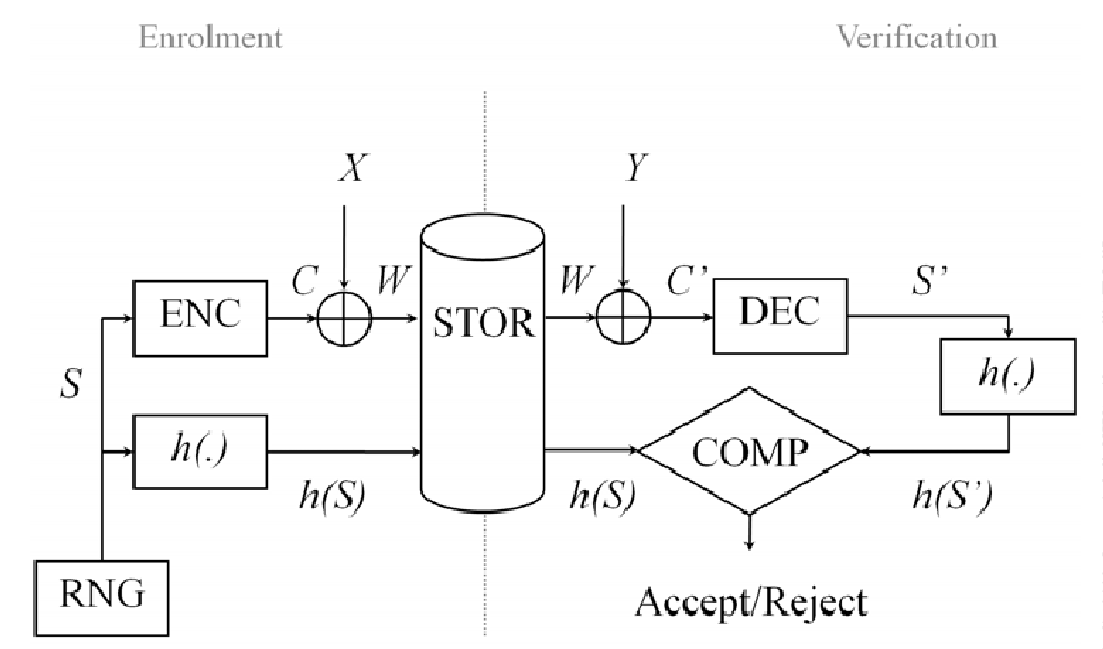
\includegraphics[width=0.85\textwidth]{img/fcs.png}
        \label{fig:fcs}
    \end{figure}
    Während der Registrierungsphase, wird ein zufälliger Schlüssel $S$ erzeugt und dessen Hashwert $h(S)$ gespeichert.
    Der Schlüssel wird um redundanten Bits ergäntzt, um eine Form von fehlerkorrigierenden Code $C$ zu erhalten (Hamming Code, 
    Reed-Solomon Code, etc.). Anschließend wird $C$ mit der biometrischen Probe $X$ binär durch eine XOR-Operation 
    verknüpft, um das Wort $W$ zu erzeugen.
    \[
        W = C \oplus X
    \]
    $W$ wird ebenfalls gespeichert.

    Während der Authentifizierung wird eine weitere biometrische Probe $Y$ gemessen. Gleicht $Y$ nun der ersten Probe $X$,
    so kann über eine XOR-Verknüpfung das Codewort $C$ wiederhergestellt werden.
    \begin{align*}
        C\oplus X \oplus Y &= C \oplus (X\oplus Y) &&\mid X = Y\\
        &= C\oplus 0\\
        &= C 
    \end{align*}
    In den meisten validen Authentifizierungsversuchen wird sich $Y$ durch die Messvariationen leicht von $X$ unterscheiden. 
    Dadurch würde man das fehlerbehaftete Codewort $C'$ erhalten, woraus dank der Fehlerkorrektur trotzdem der Schlüssel
    $S$ generiert werden kann. Zuletzt wird der Hashwert des errechneten Schlüssel mit dem gespeicherten verglichen.
    Bei Gleichheit wird akzeptiert, sonst abgelehnt.

    \section{Aufgabe 9}
    \textit{Implementieren sie das Fuzzy Commitment Scheme mit Hilfe von Hamming ECC
    (gerne library verwenden für letzteres). Als binäres biometrisches Template generieren 
    sie ein zufälliges binäres Muster, der Schüssel soll 128 Bits lang sein. Die
    biometrische Varianz simulieren sie durch Kippen einiger Bits. Dokumentieren sie
    den korrekten Key-release trotz biometrischer Varianz.}\vspace*{1em}\newline
    Für Implementierung des Fuzzy Commitment Schemes wurde die Programmiersprache Rust verwendet. Ein 128-Bit langer
    Schlüssel wird zufällig erzeugt und in ein Byte-Array mit dem Namen \verb|key| gespeichert. Außerdem wird 
    der Hashwert berechnet und der Hamming Code generiert.
    \begin{verbatim}
let key = encryption::generate_key_128();
let key_hash = hash(&key);    
let hamming_code = hamming::encode(&key)
    .expect("Failed to encode key");
    \end{verbatim}
    Dadurch enstanden in einem Versuch folgende Werte für den Schlüssel $S$ und den Hamming Code $C$:
    \begin{center}
        \begin{tabular}{cl}
            Variable & Hexadezimal Werte\\\hline
            $S$ & \verb|BC4F553EF28ED254DDB3E73605894457|\\
            $C$ & \verb|77C57AA9FBCA3B49A9BB67CE6C0B128957|
        \end{tabular}        
    \end{center}
    Man kann erkennen, dass das Codewort $C$ um zwei Stellen länger ist, als der Schlüssel $S$, weil durch den 
    Hamming Code genau 8 Paritätsbits hinzugefügt wurden. Das entspricht einem Hamming(136, 128) Code. 
    
    Als nächstes wird eine biometrische Probe $X$ zufällig generiert, wobei die Länge an die Code-Größe angepasst wird.
    Die erzeugte Probe $X$ wird danach mit dem Codewort $C$ kombiniert, um $W$ zu erhalten. 
    \begin{verbatim}
let x = rng().random_iter()
    .take(hamming_code.len())
    .collect::<Vec<u8>>();
let w = fuse(&hamming_code, &x);
    \end{verbatim}
    \begin{center}
        \begin{tabular}{cl}
            Variable & Hexadezimal Wert\\\hline
            $X$ & \verb|2E162EEF2F66DAC34B3B09A96D129F56EA|\\
            $W$ & \verb|59D35446D4ACE18AE2806E6701198DDFBD|
        \end{tabular}
    \end{center}
    Die \verb|fuse|-Funktion iteriert über jedes Byte der beiden Variablen und verknüpft sie mittels XOR.
    \begin{verbatim}
fn fuse(x: &[u8], y: &[u8]) -> Vec<u8> {
    x.iter().zip(y.iter()).map(|(&a, &b)| a ^ b).collect()
}
    \end{verbatim}
    Im zweiten Teil wird die Probe $X$ zufällig mutiert, indem ein Bit geändert wird. Dadurch soll ein 
    Authentifizierungsversuch simuliert wird, bei dem Messvariationen aufgetreten sind, das biometrische Material
    aber grundsätzlich übereinstimmt. Die erzeugte Probe $Y$ wird anschließend mit den Helferdaten $W$ zu $C'$ kombiniert.
    \begin{verbatim}
let y = random_bit_flip(&x);
let c = fuse(&w, &y);
    \end{verbatim}
    \begin{center}
        \begin{tabular}{cl}
            Variable & Hexadezimal Wert\\\hline
            $Y$ & \verb|2E162EEF2F66DAC34B3B09A96D129F5EEA|\\
            $C'$ & \verb|77C57AA9FBCA3B49A9BB67CE6C0B128157|
        \end{tabular}
    \end{center}
    Zuletzt wird das Codewort $C'$ fehlerkorrigiert, um die Veränderungen auszugleichen und den Schlüssel $S'$ 
    herzustellen. Stimmt der Hashwert dieses Schlüssel mit dem ursprünglichen von $S$ überein, so war die 
    Authentifizierung erfolgreich, ansonsten nicht.
    \begin{verbatim}
let s = hamming::error_correct(&c);

let auth_hash = hash(&s);
if auth_hash == key_hash {
    println!("Authenticated");
} else {
    println!("Not authenticated");
}
    \end{verbatim}
    Man erkennt an diesem Beispiel gut, dass zu keinem Zeitpunkt der ursprüngliche Schlüssel gespeichert werden muss und nur 
    Anfangs zur Berechnung von $h(S)$ und $C$ gebraucht wird. Im Speicher liegen also nur $W$ und $h(S)$, woraus weder
    die biometrischen Daten noch der Schlüssel errechnet werden können. Der vollständige Quellcode des Beispiels
    ist auf GitHub\footnote{\href{https://github.com/Andino20/cryptoS25/tree/main/blatt02/fcs}{https://github.com/Andino20/cryptoS25/tree/main/blatt02/fcs}} zu finden.
    \newpage
    \bibliographystyle{plainnat}
    \bibliography{refs}
\end{document}